%! Author = chicken1925
%! Date = 2020/10/16

% Preamble
\documentclass[11pt]{article}

% Packages
\usepackage{amsmath}
\usepackage[dvipdfmx]{graphicx}

% Document
\begin{document}
    2119116s 佐野 海徳\\
(1).a)リスク資産だけの収益率を$R_p$ 、無リスク資産の収益率を$r_f$ 、当初リスク資産に投資した割合をx、全体の収益率を$R_{xp}$,リスク資産を増やしたときの割合をy、全体の収益率を$R_{yp}$とする。
このとき$ E[R_{xp}] = (1 - x)r_f = xE[R_p] = r_f + x(E[R_p] - r_f)$, $E[R_{yp}] = (1 - y)r_f + xE[R_p] = r_f + y(E[R_p] - r_f)$となる。
ここで$x < y$であるのと明らかに無リスク資産の期待リターンよりリスク資産の期待リターンのほうが大きいことから$E[R_{xp}] < E[R_{yp}]$となる。
\par 無リスク資産の利子率は一定で、ポートフォリオの動きに関係なく利益を出せるので分散もリスク資産との共分散も0である。ここで分散をV、共分散をCOVとおくと $V(R_{xp}) = (1 - x)^2 V(r_f) + x^2 V(R_p) + 2(1 - x)x + COV(r_f,R_p) = x^2 V(R_p)$。
$R_{yp} = y^2 V(R_p)$であるから、分散は大きくなる。\\
(1).b) iを加えたときもjを加えたときも、どのように変化するかはそのポートフォリオが現在どのような性質を持っているかに左右されるので、i,jの追加による変化には直接の関係はない。\\
(1).c) この条件のもとでは、個々の証券のリスクそのものではなく、市場ポートフォリオのリスクに影響を与える度合いが評価の尺度となる。CAPMの式より、個々のリスク資産をi,市場ポートフォリオをMとすると$E[r_i] - r_f = \frac{E[r_M] - r_f}{V[r_M]}COV[r_i,r_M]$となり、左辺に影響を与える変数たりえるのは$COV[r_i,r_m]$だけだからである。\\
このとき、このCAPMの式は${\beta}_i = \frac{COV[r_i,r_M]}{V[r_M]}$としたときに$E[r_i] - r_f = {\beta}_i{R[r_M] - r_f}$と変形される。また、$COV[r_M,r_M] = 1$である。縦軸を期待リターン、横軸をベータとしたときにこの式は無リスク資産だけに投資した場合の点(ベータ = 0)と市場ポートフォリオを表す点(ベータ = 1)を通る直線上にすべてのリスク資産が乗っているということを示していて、
この式で表される直線が証券市場線と呼ばれる直線である。\\
(2).a)2ページ目上部に挿入されている。\begin{figure}[ht]
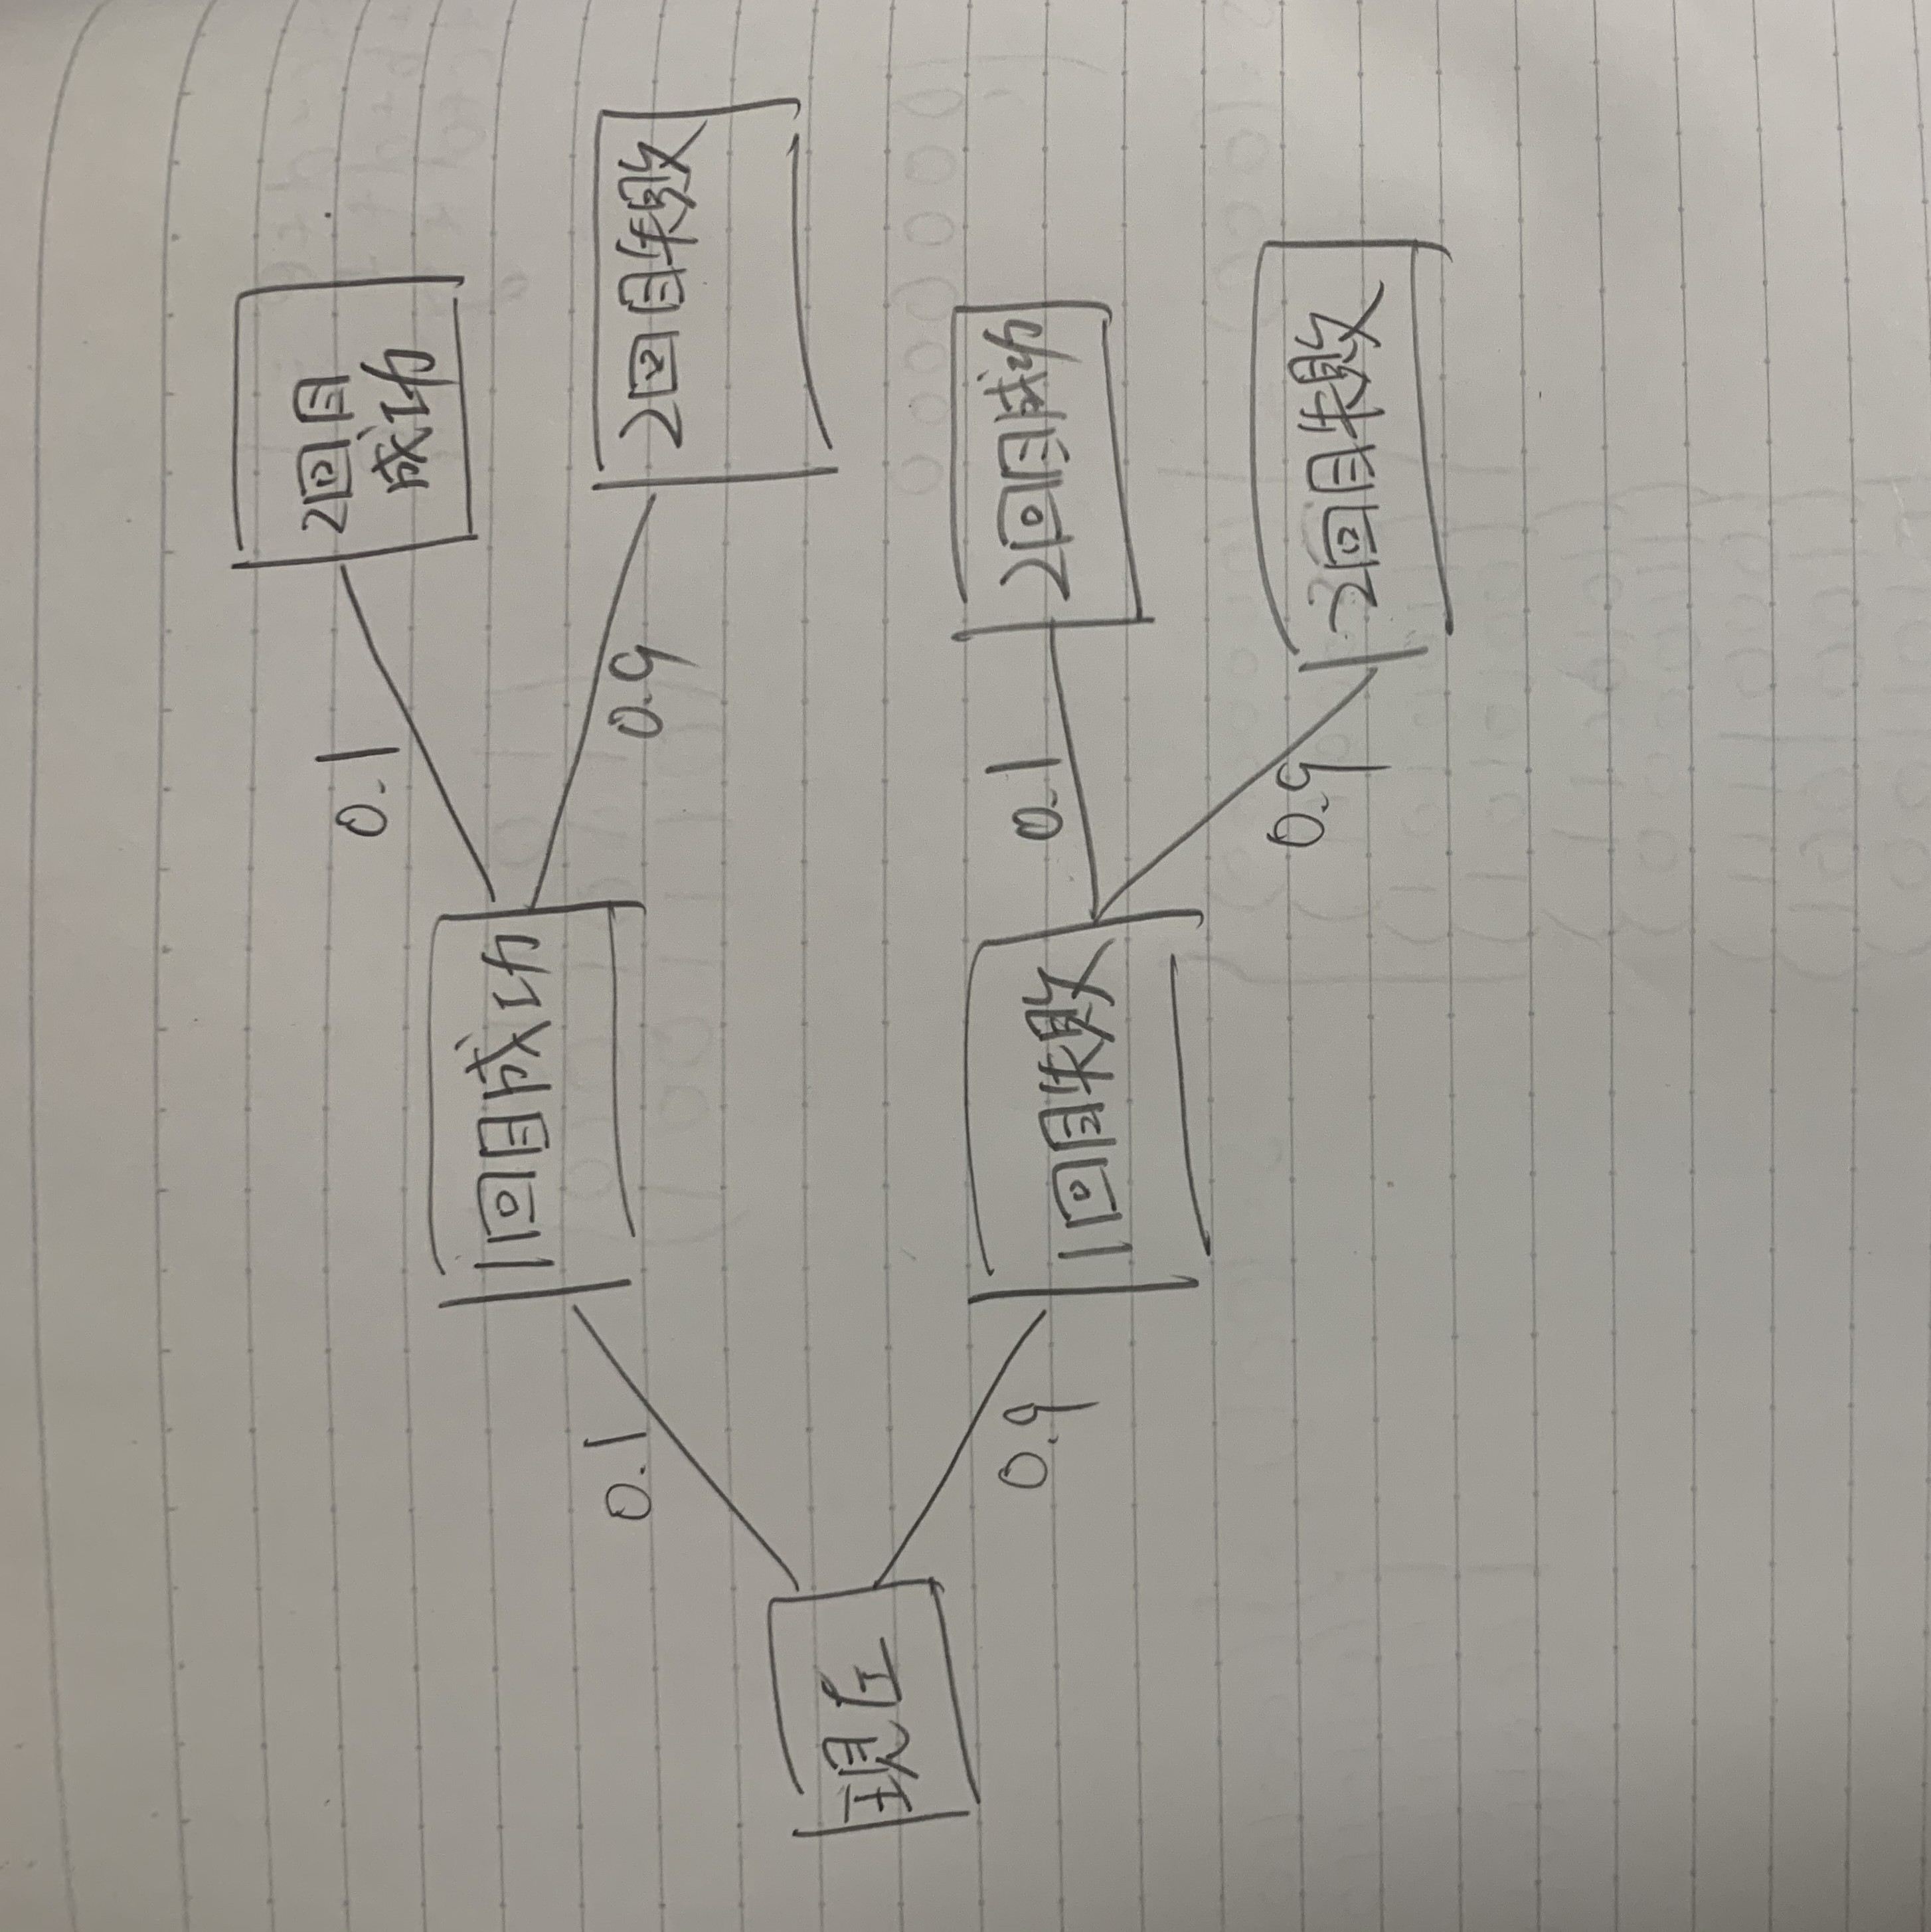
\includegraphics[height = 8cm,width= 80mm,angle = -90]{IMG_2214.JPG}
\end{figure}
(2).b)Covid-19の臨床テストで成功した場合、特許料は10\%で100億円、90\%で60億円になる。よって求める期待値は$100 \times 0.1 + 60 \times 0.9 = 10 + 54 = 64$(億円)である。
最初のテストで失敗した場合、特許料は10\%で20億円、90\%で0円になる。よって求める期待値は$20 \times 0.1 + 0 \times 0.9 = 2$(億円)である。\\
(2).c) a)ではその地点でどう価格が変動するかがその地点ですべてわかっているから期待値が通常の計算で求められるが、テストの成功、失敗によって最終的な価格がどうなるかは現在をtとしたとき、t + 1地点、つまり1回目の実験の結果がわからないと不明だから、価格変化は予測できず価格変化は予測できない。よって
期待値は0。\\
(2).d) b)で期待値を求めたときは授業資料における繰り返し期待の法則(1)を用いている。そこでの操作しか最終的に取り得る価格に影響しないため、この操作における期待値は情報集合Iを\{成功、失敗\} = \{0.1,0.9\}と表したときの合理的な期待値となる。
c)で期待値を求める際は現在の情報集合が${\omega}_0$ = \{成功,失敗\}であるのに対し、一回目のテストで成功したときの情報集合は${\omega}_{1s} = $ \{1回め成功,1回め成功$\to$2回目成功,1回め成功$\to$2回め失敗\}であり、一回目のテストで失敗したときの情報集合は
${\omega}_{1f} =$ \{1回め失敗,1回め失敗$\to$ 1回め失敗, 1回め失敗$\to$ 2回め成功\}であるから、${\omega}_0 \subset {\omega}_{1s}$かつ${\omega}_0 \subset {\omega}_{1f}$だから、c)の結果の導出には講義資料の繰り返し期待の法則の(3)を仮定とした(4)が成り立っている。\\
(2).e)
(3).a)n銘柄の株式からなる等ウェイトポートフォリオの分散をVとするとVは$\frac{1}{n}$(個々の株式の分散の平均) + $1 - \frac{1}{n}$(株式間の共分散の平均)で表される。$\lim_{n \rightarrow \infty}V=$(株式間の共分散の平均)である。
よって求める値は$\sqrt{V} = \sqrt{\frac{2}{3} \times 0.30 \times 0.30} \simeq 24 \% $である。\\
(3).b)${\delta}^2_{i} = E[{r_{i} - E(r_{i})}] = E[{({({\alpha}_{i} + {\beta}_ir_M +{\epsilon}_i})}^2] = E[{\beta_i(r_m - E(r_m) + {\epsilon}_i) - E({\alpha}_i + {\beta}_ir_M + {\epsilon}_i)}^2]$\\
$= {\beta}^2_iE[{(r_M - E(r_M))}^2] + 2{\beta}_iE[{(r_M - E(r_M))({\epsilon}_i - E({\epsilon}_i))}] + E[{{\epsilon}_i - E({\epsilon}_i)}^2] = {\beta}^2_i{\delta}^2_m + 2{\beta}_iCOV[r_m,{\epsilon}_i] + {\delta^2}_{\epsilon} = {\beta}_i{\delta}_m + {\delta}_{\epsilon}$\\
ここで、${\delta}_{\epsilon}$は個別株式の分散に等しい。このとき、右辺第一項は0になるので計算すると完全に等式が成り立つ。したがってこの例では個別株式の期待リターンの分散は100\%説明される。\\
(3).c) ($\rm(\hspace{.18em}i\hspace{.18em})$)求める割合はリスク資産の期待超過リターンとその分散の比率を相対的リスク回避度で割ったものであるから$\frac{1}{2} \frac{\frac{6}{100}}{\frac{9}{100}} = \frac{1}{3}$。\\
($\rm(\hspace{.08em}ii\hspace{.08em})$)期待値を取れば良いので求めるリターンをRとして$R = \frac{1}{3} \times \frac{6}{100} + \frac{2}{3} \times \frac{3}{100} = \frac{1}{50} + \frac{1}{50} = \frac{1}{25} = 4(\%)$。\\
($\rm(i\hspace{-.08em}i\hspace{-.08em}i)$)分散を求めると$\frac{1}{2}{(0.04 - 0.03)^2 + (0.04 - 0.06)^2} = 0.00025$なので、求める標準偏差は0.0158....$\sim 1.6\%$である。\\
(3).d)



\end{document}